% #############################################################################
% This is Appendix B
% !TEX root = ../main.tex
% #############################################################################
\chapter{Sefl-supervised learning as feature extractor for children's ASR}
\label{chapter:appendixB}

\section{Introduction}
% Very short intro SSL
In light of the increasing availability of large amount of unlabeled speech data, there has been a need to efficiently extract general-purpose knowledge from it. Consequently, SSL has experience notable advances and has gained substantial attention in recent years especially in the context of low-resource tasks. SSL refers to a training paradigm where a model learns representations from unlabeled speech data without relying on explicit labels or annotations. This approach yields discernible enhancements in performance across various applications such as speech recognition, speaker identification, and emotion recognition \cite{baevski2020wav2vec}. Traditionally, SSL models can be used in two manners: firstly, as a feature extraction to replace human-designed features \cite{yang21c_interspeech,chang2021exploration}, and secondly, as a model initialisation accomplished by concatenating prediction layers and fine-tuning the entire model \cite{fan2022draft,jain2023wav2vec2,wang2021fine,li2021accent}.

% Children ASR SSL
In recent years, an incrase number of research focus on using SSL models for children ASR. One notable avenue observed in the literature involves the fine-tuning of SSL models exclusively using children's data \cite{jain2023adaptation} or through a combination of adult and children's data \cite{jain2023wav2vec2}. These efforts have yielded improved performances, showcasing the adaptability of SSL models to the nuances inherent in the speech patterns of children. Conversely, an alternative strategy has emerged by using Adapters to adapt SSL models specifically to children's speech characteristics subsequently followed by the full model, Adapters included, fine-tuning \cite{fan2022draft}. This initial training, allow to reduce the complexity associated with the conventional process of fine-tuning the entire model directly with children speech.
%  Our motivation
The observed successes of SSL as an initialisation for fine-tuning in the context of children's ASR underscore its efficacy as a new training paradigm. However, the exploration of SSL models as front-end feature extractors, compared to the conventional hand-crafted features, despite its use and success for adult speech \cite{yang21c_interspeech,chang2021exploration} remains unexplored for childen's ASR. Motivated by these considerations, this chapter undertakes a comprehensive review of various SSL models, evaluating their potential as novel feature extractors in the domain of children's ASR.
\section{Self-supervised pre-trained models}

\begin{table}[htbp]
    \centering
    \begin{tabular}{ccccccc}
      \toprule
      Method & Architecture & \#Params & Stride & Input & Corpus & \\%Pretraining \\ 
      \midrule
      FBANK & - & 0 & 10ms & waveform & - & \\%- \\
      Mockingjay \cite{mockingjay} & 12-Trans & 85.12M & 10ms & FBANK & LS 360 hr \\%& 360 hr time M-G \\
      Audio ALBERT \cite{chi2021audio} & 3-Trans & 7.15M  & 10ms & FBANK & LS 960 hr \\
      NPC  \cite{liu21l_interspeech} & 4-Conv, 4-Masked Conv & 19.38M & 10ms & FBANK & LS 360 hr \\%& 360 hr M-G + VQ \\
      APC \cite{chung19_interspeech} & 3-GRU & 4.11M & 10ms & FBANK & LS 360 hr \\%& 360 hr F-G \\
      TERA \cite{liu2021tera} & 3-Trans & 21.33M & 10ms & FBANK & LS 960 hr\\%& 960 hr time/freq M-G \\
      wav2vec 2.0 Base \cite{baevski2020wav2vec} & 7-Conv, 12-Trans & 95.04M & 20ms & waveform & LS 960 hr\\%& 960 hr M-C + VQ \\
      wav2vec 2.0 Large \cite{baevski2020wav2vec} & 7-Conv, 24-Trans & 317.38M & 20ms & waveform & LL 60k hr\\%& 60k hr M-C + VQ \\
      Distill HuBERT \cite{chang2022distilhubert} & 7-Conv, 3-Trans & 23.49M & 20ms & waveform & LS 960 hr \\%& 960 hr M-P + VQ \\
      HuBERT Base \cite{hsu2021hubert} & 7-Conv, 12-Trans & 94.68M & 20ms & waveform & LS 960 hr \\%& 960 hr M-P + VQ \\
      HuBERT Large \cite{hsu2021hubert} & 7-Conv, 24-Trans & 316.61M & 20ms & waveform & LL 60k hr\\%& 60k hr M-P + VQ \\
      \bottomrule
    \end{tabular}
    \caption{Overview of different SSL architectures used in this chapter}
    \label{tab:SSL_models}

  \end{table}


Traditionally, SSL models can be categorised into two distinct approaches: generative modeling and discriminative modeling. In this section, we will focus on summarising a selection of SSL models, presented in Table \ref{tab:SSL_models}, with a particular emphasis on their differences.

\subsection{Generative modeling}
% List a couple of model and explain their differences
Generative modeling has emerged as a prevalent approach for learning speech representations for SSL. Generally, generative models are trained to generate speech frames based on their learned speech representations with or without the help of context. For instance, the Autoregressive Predictive Coding (APC) model \cite{chung19_interspeech} adopts a language model-like training paradigm, where a Recurrent Neural Network (RNN) generates future frames predicted from the past frames. 
The Mockingjay model \cite{mockingjay} takes inspiration from BERT-like pretraining techniques by masking input acoustic features along the time axis and subsequently regenerating the masked frames while the Audio ALBERT represent a smaller version of it \cite{chi2021audio}. Expanding upon this concept, the Temporal Encoder Representations from Acoustics (TERA) model \cite{liu2021tera} introduces an additional layer of complexity by masking bins in the frequency axis alongside the temporal axis. Finally, the Non-autoregressive Predictive Coding (NPC) model \cite{liu21l_interspeech} combines elements from both APC and Mockingjay by substituting the RNN in APC with a CNN layers and modifying the future frames generation process into a masked reconstruction.

\subsection{Discriminative modeling}
\begin{figure}[t]
    \centering
    \subfigure[Illustration of the Wav2vec2 architecture taken from \cite{baevski2020wav2vec}]{\label{fig:wav2vec2}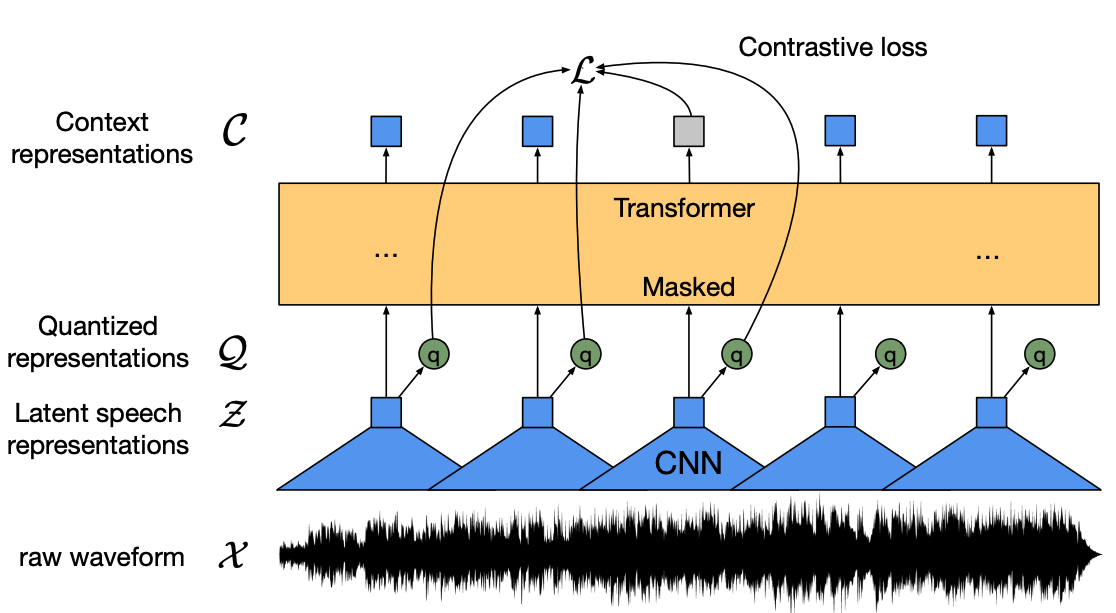
\includegraphics[width=0.48\textwidth]{imgs/wav2vec2.png}}
    \subfigure[Illustration of the HuBERT architecture taken from \cite{hsu2021hubert}]{\label{fig:Hubert}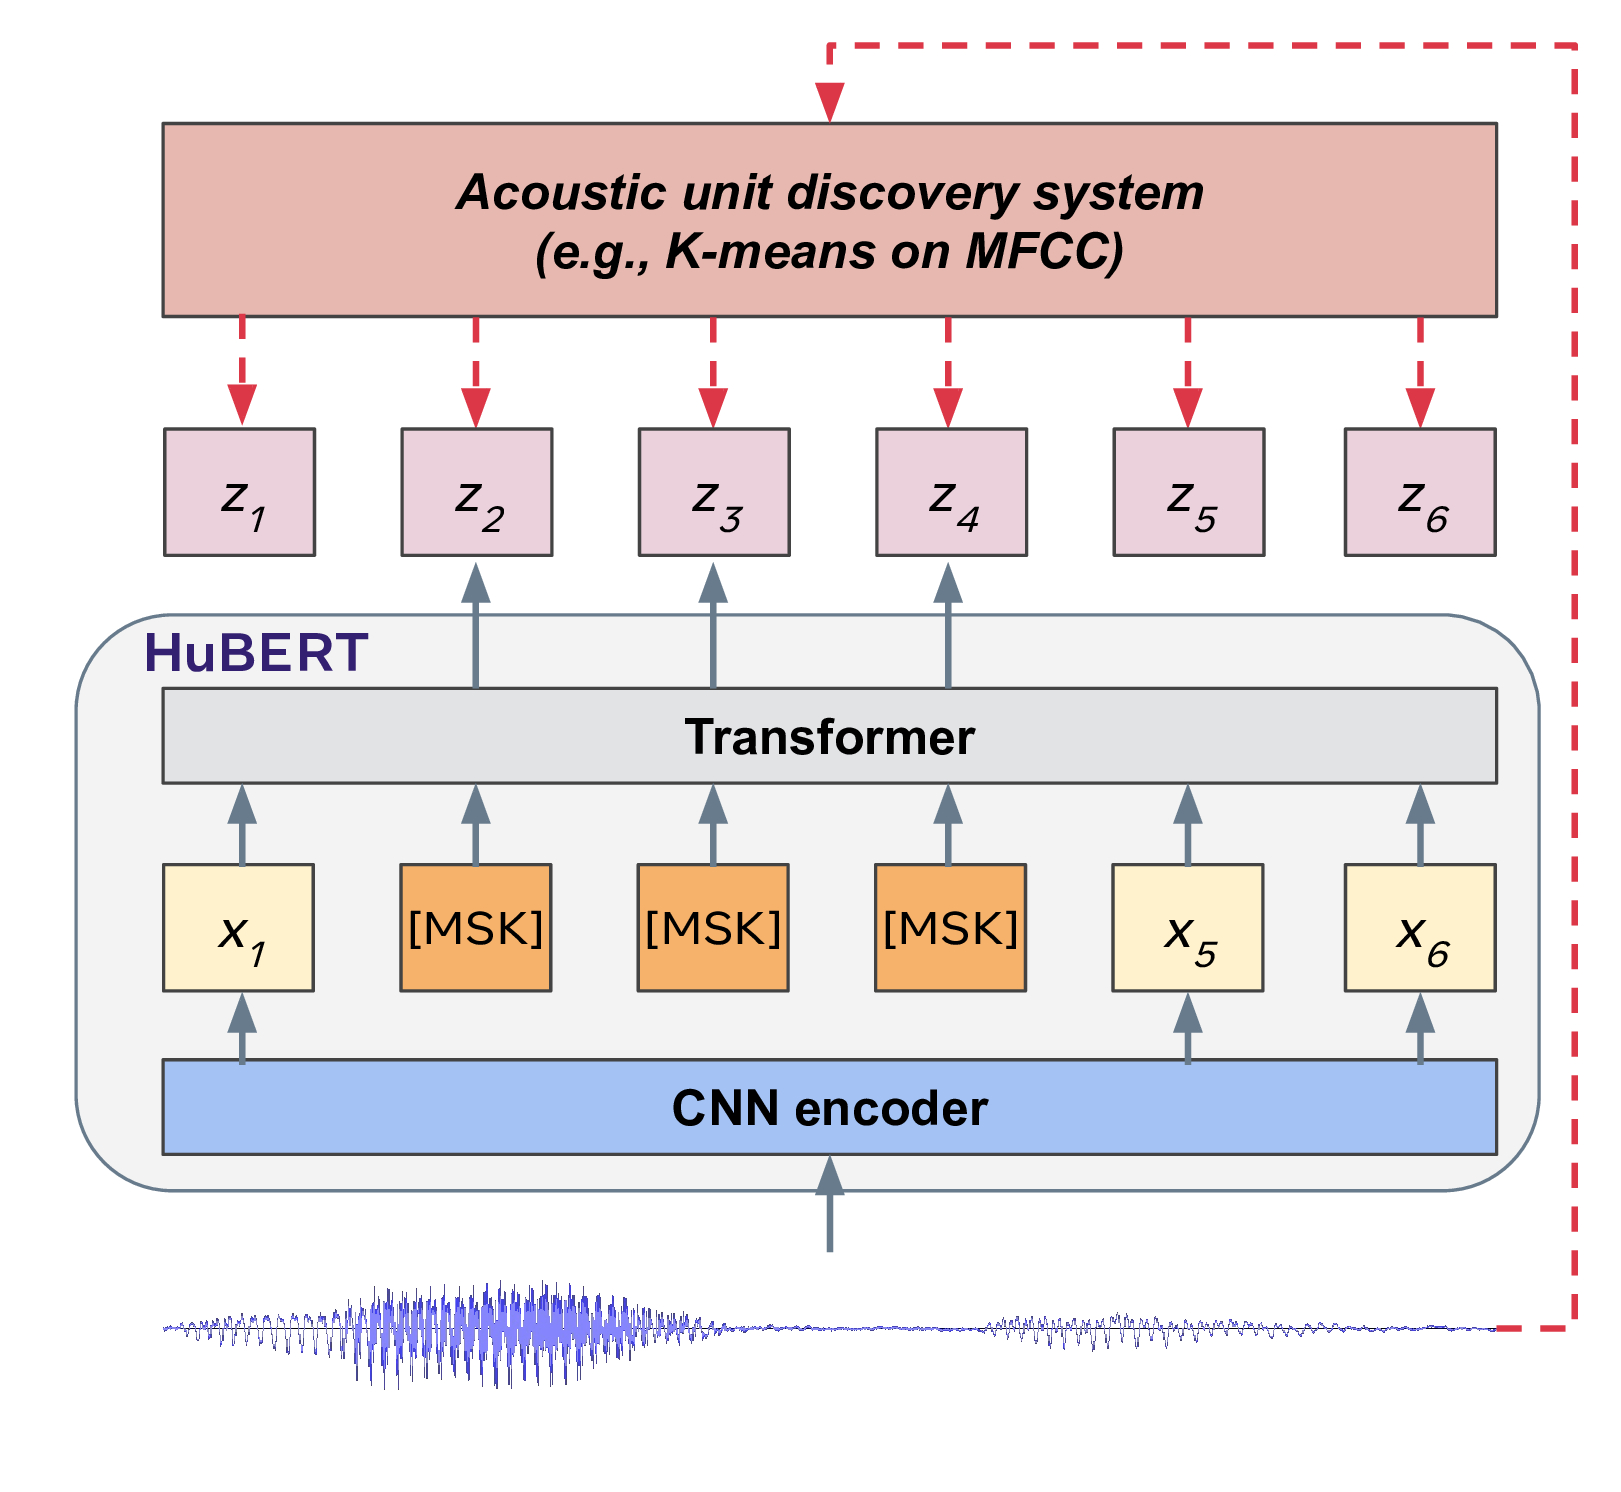
\includegraphics[width=0.48\textwidth]{imgs/Hubert.png}}
    \caption{Overview of the discriminative SSL Wav2vec2 and HuBERT models}
\end{figure}
% Explain Wav2Vec2 and Hubert    
The success of discriminative modeling has been notably pronounced with the introduction of the contrastive loss, a technique where the model discerns between correlated positive samples and negative samples. The underlying intuition is that positive samples should exhibit closer representations in comparison to their negative counterparts. A prominent exemplar of this approach is evident in the Wav2Vec2 model \cite{baevski2020wav2vec}, which has demonstrated promising potential in learning speech representations. The Wav2Vec2 model achieves this by masking latent representations of the raw waveform and formulating a contrastive task over quantized speech representations. A more detailed representation of Wav2Vec2 architecture is displayed in figure \ref{fig:wav2vec2}. Later, moving away from the contrastive loss, the work of \cite{hsu2021hubert} proposed the HuBERT model. This model introduces a novel methodology by incorporating BERT's token prediction via offline clustering on representations. Specifically, the HuBERT model use a BERT-like training that consumes masked continuous speech features to predict pre-determined cluster assignments. The labels assigned to the masked locations during clustering serve as the predicted targets. Importantly, the predictive loss is selectively applied solely over the masked regions, compelling the model to learn robust high-level representations of unmasked inputs in order to accurately infer the targets of the masked ones. The HuBERT architecture is shown in figure \ref{fig:Hubert}. An distilled version of the HuBERT is also explored in our experiments \cite{chang2022distilhubert}.
\section{Experimental setup}
In our experimental setup, we used the Self-Supervised Speech Pre-training and Representation Learning (s3prl) toolkit\footnote{https://github.com/s3prl/s3prl}. The s3prl allow the modular use of pre-trained SSL models, called upstream, to perform various downstream tasks. In order to evaluate the efficiency of different SSL models as features extractor for children's ASR, we froze the pre-trained models's weight to extract embedding representation of the speech signal as new acoustic features. All the differents SSL upstream models used in our experiments are listed along with detailed informations regarding their architectures in table \ref{tab:SSL_models}. Notably, each of these models underwent self-supervised pre-training on either 360 or 960 hours of LibriSpeech \cite{librispeech} (denoted as LS 360hr and LS 960hr, respectively) or on an extensive 60 thousand hours of LibriLight data \cite{librilight} (referred to as LL 60k hr) . 
The ASR downstream task was conducted using a 2-layered Bidirectional Long Short-Term Memory (BiLSTM) architecture with 1024 units, optimised with a CTC loss. The training spanned 800 thousand iterations, with a learning rate set at $1.0\dot 10^{-4}$. Additionally, a dropout rate of $0.2$ was applied to the BiLSTM architecture to increase robustness. Limited by the large size of some SSL model, we decided to used a subset of the Myst \cite{MyST} dataset, using 77 hours of speech for training, by removing the longest utterances in the train and validation sets. A detailed description of the filtered Myst data is provided in table \ref{tab:ssl_myst}.
\begin{table}[h!]
    \caption{My Science Tutor Children Speech Subset Corpus statistics}
    
    \begin{center}
    \begin{tabular}{r|ccc}
    \hline
     & Training & Validation     & Test   \\ \hline
    \# of utterances & 23594   & 3959    & 4079  \\ 
    \# of speakers & 559  & 79    & 91  \\ 
    \# of hours & 77   & 12    & 13  \\ \hline
    \end{tabular}
    \label{tab:ssl_myst}
    \end{center}
    \end{table}


\section{Results}

%For these models, the training process is separated into two stages. The first phase of training is self-supervised, which implies that no labels are used during training. The objective of this first phase is to present a large amount of unlabelled data to the system so that it learns a good speech representation. The second stage of learning is supervised fine-tuning, in which the model is taught to predict specific phonemes using the robust representation acquired in the previous stage with the help of a small amount of labelled data.
%In this category, two models stand out as state-of-the-art: Wav2Vec 2.0 \cite{baevski2020wav2vec} and HuBert \cite{hsu2021hubert}. As a preliminary experiment, to asses the usability of such frameworks for children ASR, we trained a BiLSTM model using the output of a variety of frozen self-supervised systems. For this experiment we used a subset of 50h of the Myst corpus \cite{MyST}, and the preliminary findings are displayed in the table \ref{tab:ssl}
%\begin{table}[ht]
%\centering
%\begin{tabular}{lcc} 
%\hline
%SSL upstream & UER $\downarrow$ & WER $\downarrow$ \\ 
%\hline
%Fbanks & 12.29\% & 35.14\% \\ 
%\hline
%Mockingjay & 12.49\% & 35.08\% \\
%APC & 11.88\% & 32.84\% \\
%TERA \cite{tera} & 11.31\% & 31.80\% \\
%Audio Albert \cite{chi2021audio} & 12.28\% & 34.69\% \\
%Wav2Vec2.0 Base & 7.37\% & 19.76\% \\
%Wav2Vec2.0 Large & 7.00\% & 18.76\% \\
%Distill HuBERT \cite{chang2022distilhubert} & 9.22\% & 25.75\% \\
%HuBERT Base & 7.40\% & 19.77\% \\
%HuBERT Large & \textbf{6.03\%} & \textbf{15.41\%} \\
%\hline
%\end{tabular}
%\caption{Results without language model of different Self-supervised models as feature extractors}
%\label{tab:ssl}
%\end{table}

\begin{table}[ht]
  \centering
  \begin{tabular}{clcc}
  \hline
  Model type                      & SSL upsteam    & UER$\downarrow$ & WER $\downarrow$ \\ \hline
  Hand-crafted                    & Fbanks         & 12.29\%                                                           & 35.14            \\ \hline
  \multirow{4}{*}{Generative}     & Mockingjay     & 12.49\%                                                           & 35.08\%          \\
                                  & Audio Albert   & 12.28\%                                                           & 34.69\%          \\
                                  & NPC   & 11.99\%                                                           & 33.07\%          \\
                                  & APC            & 11.88\%                                                           & 32.84\%          \\
                                  & TERA           & 11.31\%                                                           & 31.80\%          \\ \hline
  \multirow{5}{*}{Discriminative} & Wav2Vec2 Base  & 7.37\%                                                            & 19.76\%          \\
                                  & Wav2Vec2 Large & 7.00\%                                                            & 18.76\%          \\
                                  & Distill HuBERT & 9.22\%                                                            & 25.75\%          \\
                                  & HuBERT Base    & 7.40\%                                                            & 19.77\%          \\
                                  & HuBERT Large   & \textbf{6.03\%}                                                   & \textbf{15.41\%} \\ \hline
  \end{tabular}
  \caption{Results without language model of different Self-supervised models as feature extractors}
\label{tab:ssl}
  \end{table}

Table \ref{tab:ssl} present the results of the comparaison between various SSL pre-trained model as feature extractors for children's ASR. We provide Unit error rate (UER) as well as WER. Fbanks are established as a baseline, yielding a UER of 12.29\% and a WER of 35.14\%. In terms of generative SSL models, TERA  and Audio Albert surpass traditional Fbanks, exhibiting improvements in both UER ,11.31\% and 12.28\% respectively and WER with 31.80\% and 34.69\% respectively. Turning to discriminative SSL, the Wav2Vec2.0 Base and Wav2Vec2 Large demonstrate substantial enhancements in performance, achieving UER values of 7.37\% and 7.00\%, and WER of 19.76\% and 18.76\%, respectively. The distilled version of HuBERT outperforms Fbanks but falls behind the Wav2Vec2 models in terms of both UER and WER with 9.22\% UER and 25.75\% WER. Finally, HuBERT Base and HuBERT Large emerge as the top-performing SSL models, boasting the lowest UER with respectively 7.40\% and 6.03\% and WER of 19.77\% and 15.41\%. We observed that the best performing models are the large discriminative pre-trained on a large amount of speech data.

The results suggest that large Discriminative models, particularly HuBERT Large, demonstrate superior performance compared to other SSL models and Fbanks as featuress extractor for children ASR. Notably, even though no language model where used in this experiment, the results are of the same order as those reported in previous the different chapters of the thesis obtained with a transformer and a transformer language model. Showing the benefic of using frozen pre-trained SSL models as feature extractor for children ASR.

\section{Analysis of the extracted features}
\begin{figure}
  \begin{center}
  \centering
  \subfigure[]{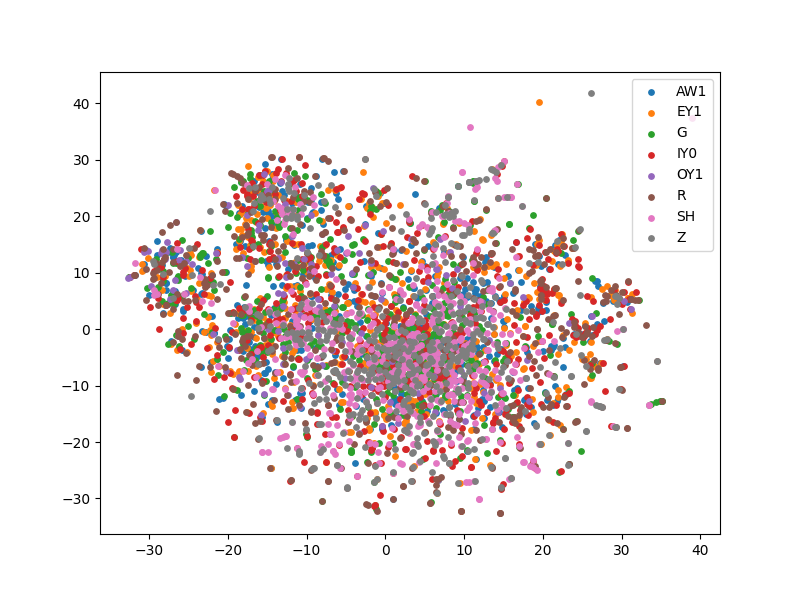
\includegraphics[width=0.49\textwidth]{imgs/fbank_umap_plot.png}} 
  \subfigure[]{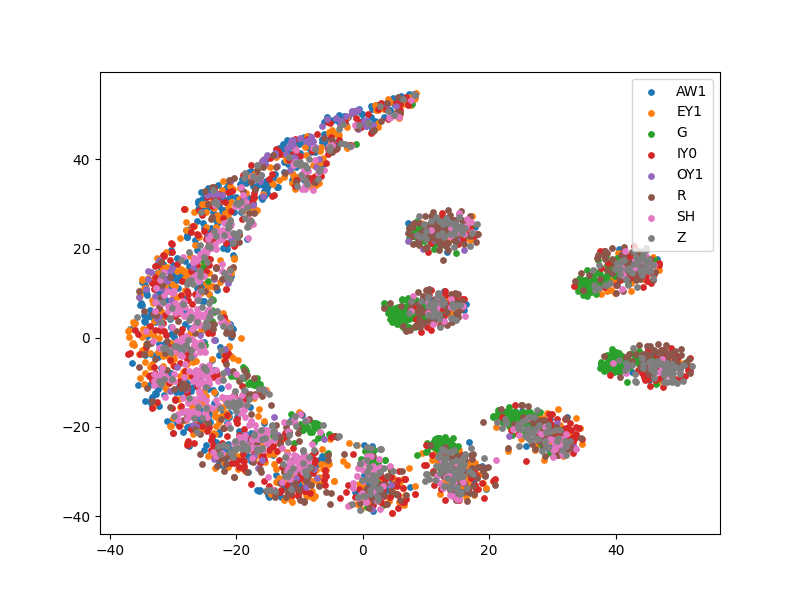
\includegraphics[width=0.49\textwidth]{imgs/tera_umap_plot.png}} 
  \subfigure[]{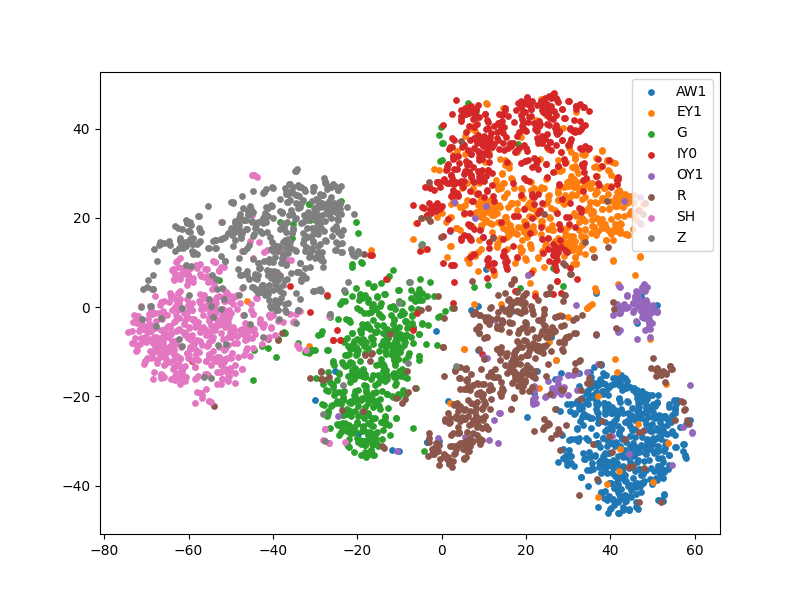
\includegraphics[width=0.49\textwidth]{imgs/wav2vec_umap_plot.png}}
  \subfigure[]{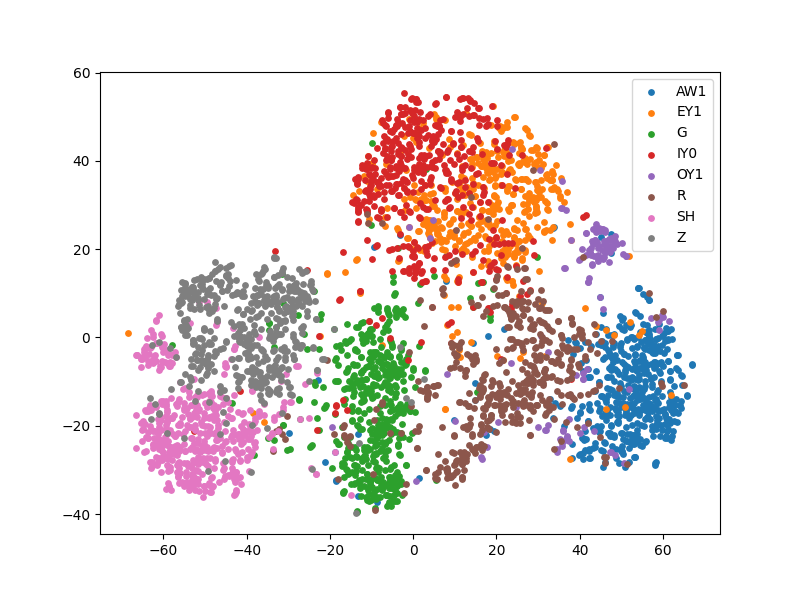
\includegraphics[width=0.49\textwidth]{imgs/hubert_umap_plot.png}}
  \caption{(a) Fbanks (b) TERA (c) Wav2Vec2 (d) HuBERT \\ T-SNE plot of the different extracted features using the same speech data using phoneme labels}
  \label{fig:tsne_ssl}  
\end{center}
\end{figure}
% Explain experiment
In this section, we delve in more detail into the distinct features extracted from various models, aiming to better understand the notable performance differences observed between Wav2Vec2 and HuBERT, in contrast to generative models like TERA and traditional filterbanks. In a first step we aligned our children's speech data to obtain phoneme alignments using the Montreal Forced Aligner \cite{mcauliffe2017montreal}. %These phoneme alignments serve as the foundation for extracting different features corresponding to each phoneme.

% Explain the plot procedure
Therefore, for each phonemes present in a utterance we obtained a variable-length feature sequences corresponding the extracted features for the different frames where the phoneme has been aligned. In order to get a single vector for each phoneme, we average these sequences. It is noteworthy that silence frames have been excluded. This operation is repeated for a subset of one thousand utterances of children speech in order to gather different exemple of the same phoneme from different speaker and different context. Subsequently, t-SNE (t-Distributed Stochastic Neighbor Embedding) plots are generated for each of the studied models. 

% Plot interpretation
The t-SNE plots are depicted in Figure \ref{fig:tsne_ssl}. We observe that traditional filterbanks features form a cloud points witn no structure. This lack of structure suggests that the fbanks features do not inherently exhibit phoneme-related information.
Moving on to the t-SNE plot for TERA features, clusters are observable, but these clusters do not align with phoneme. This observation indicates that while TERA features capture information from speech, they not encode phoneme-specific information, as evidenced by the presence of mixed phonemes within the different clusters.
In contrast, both Wav2Vec2 and HuBERT exhibit highly similar plots, wherein distinct clusters corresponding to different phonemes are evident. This finding suggests that the features extracted from Wav2Vec2 and HuBERT inherently capture phonemic information, even though no explicit phoneme annotations were provided during training. The presence of these phoneme-related clusters indicates that the usage of these features facilitate the ASR task by implicitly encoding phoneme information.



\section{Conclusions and future work}
% Conclusion 

% Careful about the language used and future work
However, it is crucial to emphasise that the outcomes and findings of our experiments are highly dependent on the language used. Specifically, all the SSL models were pre-trained using English language, which align with the language of the children dataset used in this experiment. Consequently, the generalisability of our results may be limited when applied to different languages. Using a different language could potentially result in decreased performances, as the SSL models may not be as adept at capturing the linguistic nuances and acoustic characteristics specific of that particular language \cite{phdthesis}. To address the language-dependent nature of our results, future work could explore the efficacy of employing multi-lingual SSL models, such as XLS-R \cite{babu2021xlsr}.
%Where Base, and Large represent the same model with different number of parameters (in the order Base $<$ Large).
%Even though we did not use a language model in this pilot experiment, the results are of the same order as those reported in section \ref{section:exp} obtained with a transformer and a transformer language model. Such results demonstrate that SSL learns substantial speech characteristics. For future research, we aim to explore in depth what information is encoded in SSL models and why they work well on children, and how we may use this knowledge to enhance children's ASR.
